\section{Les arbres de décisions}

Deux techniques de classification par les arbres ont été dévéloppées au
début des années 1980 par deux groupes de chercheurs.
Le premier groupe, dirigé par J Ross Quinlan, a développé un algorithme d'arbres
de décision en 1986 appelé ID3. Plus tard en améliorant plusieurs 
caractéristiques de ID3, il a développé et présenté C4.5.
L. Breiman, J. Friedman, R. Olshen, et C. Stone, un groupe de statisticiens, 
ont développé un algorithme pour produire des arbres de décision binaires 
appelé CART (Classication and Regression Trees) de leur côté. Ces algorithmes
ont été le début de la recherche sur la classification par les arbres de
décisions.  Les deux approches suivent le paradigme \og Diviser pour régner \fg

Plusieurs objectifs concourent à la construction d'un arbre de décision. Ce
sont:
\begin{itemize}
  \item Une meilleure généralisation des exemples de la base d'apprentissage.
  \item Une meilleure classification de nouveaux exemples
  \item Une structure aussi simple que possible
\end{itemize}
La construction d'un arbre de décision consiste à partitionner un ensemble de 
données en des groupes les plus homogènes possible du point de vue de la 
variable à prédire. On prend en entrée un ensemble de données classées, et on 
fournit en sortie un arbre. Nous obtenons un arbre qui représente une série de 
noeuds en plaçant dans la partie supérieure le noeud dont la capacité de 
classification est la plus grande. \cite{criminisi2011} 
Le résultat final est un arbre renversé comme celui représenté dans la figure
\ref{fig:DecisionTree}

\begin{figure}[h!]
  \begin{center}
    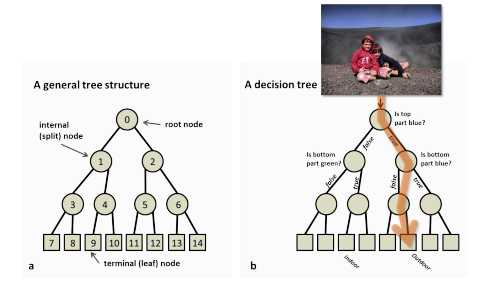
\includegraphics[width=14cm]{images/decisionTree.png}
    \caption{Arbre de décision. 
	\label{fig:DecisionTree}}
  \end{center}
  \textit{Le $a$ représente la structure générale d'un arbre de décision. Le
$b$ montre un arbre de décision illustratif utilisé pour déterminer 
si une photo représente une scène d'intérieur ou d'extérieur.}
\end{figure}

\subsection{Structure d'un arbre de décision}

Le fonctionnement des arbres de décisions repose sur les heuristiques 
construites sur des techniques d'apprentissage supervisées.

Les arbres de décisions sont composés de noeuds et de feuilles reliés par des
branches. Dans leur représentation graphique la raçine est placée tout en haut
et les feuilles en bas. Les noeuds internes sont appelés des noeuds de décision.
Ils peuvent contenir une ou plusieurs règles. Les noeuds terminaux contiennent
la classe aussi appelée classe à prédire ou étiquette. Après sa construction, un
arbre de décision peut être traduit par un ensemble de règle.

L'algorithme  générique  de construction d'un arbre permet de générer
itérativement l'arbre en prenant à chaque itération une variable et en lui
créant ses noeuds et ses feuilles. L'idée centrale est la suivante:

\textit{Diviser récursivement et le plus efficacement possible les exemples de  
l'ensemble d'apprentissage par des tests définis à l'aide des attributs
jusqu'à ce que l'on obtienne des sous-ensembles d'exemples ne contenant 
(presque) que des exemples ayant tous la même étiquette.}

 \subsection{Optimisation des noeuds}
 
 En général, on décide qu'un noeud est terminal lorsque tous les exemples
 associés à ce noeud, ou du moins  la plupart d'entre eux ont la même étiquette
 ou s'il n'y a plus d'autres caractéristiques non utilisées dans la branche
 correspondante.

 La sélection d'un test à associer à un noeud pour obtenir un arbre optimal 
 est un choix crucial. En effet, construire un arbre de décision optimal
 consiste à construire un arbre de décision le plus petit possible rendant compte
 au mieux des données. Il s'agit donc de rechercher le test qui permet de faire
 évoluer la tâche de classification. Pour mesurer cette évolution, \textit{CART}
 utilise l'\textit{indice de Gini}. Les algorithmes de Quinlan eux, utilisent  la
 notion d'\textit{entropie}.

 \subsubsection{Entropie de Shannon}

L'entropie de Shannnon correspond à la quantité d'information fournies par un
évènement: plus la probabilité d’un événement est faible (il est rare), plus 
la quantité d’information qu’il apporte est grande. Sa formule est la
suivante
\cite{benjamin2005}:
$$  
Entropie = - \sum_{i=1}^{n} {p_i * log_2(p_i)}
$$ 
Tel que $p_i$ est la proportion d'exemples de S ayant pour classe résultante
(étiquette) $i$. 

Pour un ensemble de données $T$ caractérisé par $n$ classes ($C_1, C_2, \cdots,
C_n$) selon la variable cible, la quantité d'information nécessaire pour
identifier la classe d'un individu correspond à l'entropie $E(P)$ où $P$est la
distribution de probabilité de la partition ($C_1, C_2, \cdots, C_n$).
$$
P = (\frac{|C_1|}{|T|}, \frac{|C_2|}{|T|}, \cdots, \frac{|C_n|}{|T|})
$$
$|C_i|$ représente le cardinal de la classe $i$ c'est-à-dire le nombre
d'éléments de la classe $i$.

L'entropie de $T$ est alors:

$$
Entropie(T) = - \sum_{i=1}^{n}{\frac{|C_i|}{|T|} log_2\frac{|C_i|}{|T|}}
$$

La fonction permettant de sélectionner le test qui doit étiqueter le noeud
courant  est la fonction \textit{Gain}. Pour un ensemble de données $T$, le gain
d'information de $T$ par rapport à une partition $T_j$ donnée est la variation
d'entropie causée par la partition de T selon $T_j$
$$
Gain(X, T) = Entropie(T) - Entropie(X, T) = Entropie(T) - \sum_{j=1}^{m} {\frac{T_j}{T} * Entropie(T_j)}
$$

Le gain permet de calculer ce que l'attribut spécifié apporte au désordre
du set. Plus un attribut contribue au désordre, plus il est important de le
tester pour séparer le set en plus petits sets ayant une entropie moins 
élevée.

\subsubsection{Indice de Gini}
L'indice de Gini est une mesure statistique permettant de rendre compte de la
répartition d'une variable au sein d'une population. Il mesure l'impureté qui
est un concept très utile dans la construction des arbres de décision: La qualité
d'un noeud et son pouvoir discriminant peuvent être évalués par son impureté.
Sa formule est la suivante:
$$
Gini(T) = 1 - \sum_{j=1}^{m}{(p_i)^2} =  1 - \sum_{j=1}^{m}{(\frac{|T_j|}{|T|})^2} 
$$




\subsection{Algorithmes d’induction d’arbres de décision}

Il existe essentiellement deux grandes familles d'algorithmes permettant de construire
des arbres de  décisions à partir d'un set de données: les algorithmes de
Quinlan (\textbf{ID3}, \textbf{C4.5}, \textbf{C5.0}) et l'algorithme
\textbf{CART}. Les deux approches suivent le paradigme \og diviser pour régner
\fg. Nous présentons ici le principe des trois algorithmes de construction des
arbres de décision que sont l'algorithme ID3, l'algorithme C4.5 et l'algorithme
CART.

%\input{sources/chapter4_arbre/generic}

   \subsubsection{CART}
  L'algorithme Classification and Regression Trees(\textit{CART}) est très
  similaire à C4.5, mais il en diffère par le fait qu’il prend en charge la
  régression en ne calculant pas des ensembles de règles. Il s'agit d'un  
  algorithme développé par Breiman, Friedman, Olshen et Stone (1984).

  Selon l'algorithme CART, un arbre de décision est construit en déterminant
  les questions (appelées fractionnements de noeuds) qui, lorsqu'on y répond,
  conduisent à la plus grande réduction de l'impureté de Gini. Cela signifie 
  que l'arbre de décision tente de former des noeuds contenant une forte 
  proportion d'échantillons (points de données) provenant d'une seule classe en
  trouvant des valeurs dans les caractéristiques qui divisent proprement les 
  données en classes(étiquettes).
 
  \subsubsection{ID3}
  Iterative Dichotomiser 3(\textit{ID3}) a été developpé par Ross Quinlan en
  1986. Il se base qur le concept d'attribut et de classe. L'algorithme 
  recherche l'attribut le plus pertinent à tester pour que l'arbre soit le
  plus court et le plus optimisé possible en déterminant l'attribut qui
  maximise le gain d'information.\cite{quinlaninduction}

  L'algorithme crée un arbre multivoie, trouvant pour chaque nœud (c'est-à-dire
  de manière gourmande) la caractéristique catégorielle qui produira le plus 
  grand gain d'informations pour les cibles catégorielles. Les arbres sont 
  cultivés jusqu'à leur taille maximale, puis une étape d'élagage est 
  généralement appliquée pour améliorer la capacité de l'arbre à généraliser 
  les données invisibles.

  \subsubsection{C4.5}
 L’algorithme \textit{C4.5} est une évolution de l’algorithme ID3. Il a 
 également été inventé par Ross Quinlan. Basé sur ID3, C4.5 possède quelques
 améliorations\cite{quinlanc45}
  \begin{itemize}
    \item Une adaptation de la fonction gain qui n'a plus tendance à aller vers
     l'attribut avec le plus de valeur possible.
    \item La possibilité de gérer les valeurs manquantes.
    \item La possibilité de post-élaguer son arbre pour éviter l'overfitting;
    \item La possibilité de manipuler des valeur continues
  \end{itemize}
  \textit{C5.0} est la dernière version de Quinlan publiée sous une licence 
  propriétaire. Elle utilise moins de mémoire et construit des jeux de règles 
  plus petits que C4.5 tout en étant plus précise.


  \begin{table}
    \begin{center}
       \renewcommand{\arraystretch}{1.5}
  \begin{tabular}{|l|c|c|}
    
    \hline
    \rowcolor[gray]{0.7}
     \renewcommand{\arraystretch}{1.5}\bf Méthode & \bf CART & \bf C4.5 \\
    \hline
    \bf{Mesure utilisé pour la sélection} & index Gini & Entropie et Gain d'info \\
    \hline
    \bf{Type des variables(attributs)} & discrètes et continues & discrètes et
    continues \\
    \hline
    \bf{Division à chaque noeud} & binaire & multiple \\
    \hline
   \end{tabular}
   \caption{Tableau comparatif des algorithmes C4.5 et CART}
    \label{tab:tab1}
  \end{center}
\end{table}



Dans le cadre de notre projet, l'algorithme qui sera utilisé pour la génération
de notre arbre de décision est \textit{C4.5}. Il permet la manipulation  de
valeurs continues et ne génère pas un arbre de décision binaire comme
\textit{CART} (tableau \ref{tab:tab1}).


Un modèle flexible  mémorise essentiellement les données d'entrainement en
les ajustant étroitement. Le problème d'un tel modèle est qu'il apprend non
seulement les relations réelles dans les données d'entrainement , mais aussi
tout bruit présent dans ces données. Un modèle rigide est dit avoir un biais
élevé parce qu’il fait des hypothèses sur les données de formation. Par
exemple, un classifieur linéaire fait l'hypothèse que les données sont linéaires
et n'a pas de flexibilité pour s'adapter à des données non linéaires.

Dans les deux cas (modèle flexible et modèle rigide), le modèle n'est pas capable de
réaliser de bonnes prédictions sur de nouvelles données.
Les arbres de décisions sont des modèles d'apprentissage flexible donc
sensible au bruit. Ils peuvent devenir très profonds c'est à dire croître
jusqu'à ce qu'il ait exactement une feuille pour chaque observation, les
classant toutes parfaitement.

Comme alternative, la forêt aléatoire empêche ce phénomne en créant des
sous-ensembles aléatoires des caractéristiques et en construisant des arbres plus
petits à l'aide de ces sous ensembles. Dans la suite nous présenterons les
forêts aléatoires une méthode supervisée d'apprentissage machine.

\section{Les forêts aléatoires}

  La forêt aléatoire est un modèle composé de nombreux arbres de décision. Plutôt
  que de se contenter de faire la moyenne des prédictions des arbres (que nous 
  pourrions appeler une \og forêt\fg), ce modèle utilise deux concepts clés qui lui 
  donnent le nom d'aléatoire:
  \begin{itemize}
    \item L'échantillonage aléatoire des données d'entrainement lors de la
      construction de l'arbre.
    \item Des sous-ensembles aléatoires de caractéristiques pour le fractionnement
      des noeuds
  \end{itemize}
  L’algorithme effectue un apprentissage en parallèle sur de multiples arbres
  de décision construits aléatoirement et entraînés sur des sous-ensembles de
  données différents. Le nombre idéal d’arbres, qui peut aller jusqu’à 
  plusieurs centaines voire plus, est un paramètre important : il est très 
  variable et dépend du problème.

  \subsection{Fonctionnement des forêts aléatoires}

  La forêt aléaoire (Random Forest) fonctionneen deux phases. La première
  consiste à créer la forêt aléatoire en combinant $N$ arbres de décisions. La
  seconde consisteà faire des prédictions pour chaque arbre créé dans la
  première phase.

  Le processus peut être expliqué dans les étapes ci-dessous:
  \begin{description}
    \item[Etape 1:] Sélectionnez k instances dans l'ensemble
      d'apprentissage.
    \item[Etape 2:] Construire les arbres de décisions associés aux points de
      données sélectionnés.
    \item[Etape 3:] Répétez les étapes 1 et 2, $N$ fois. ($N$ étant le nombre d'arbres
      de la forêt)
    \item[Etape 4:]Pour une nouvelle instance de données, trouvez la
      prédiction de chaque arbre de décision de la forêt et attribuez
      l'étiquette qui remporte la majorité des votes.
  \end{description}

  Supposons qu'il existe un ensemble de données contenant plusieurs images de
  fruits. Cet ensemble de données est attribué à un modèle de forêt aléatoire.
  L'ensemble des données est alors divisé en sous-ensemble et donné à chaque
  arbre de décision. Pendant la phase d'apprentissage, chaque arbre de décision
  produit résultat de prédiction. Lorsqu'une nouvelle instance apparaît, le
  modèle prédit la décision finale.

  \begin{figure}[h!]
    \begin{center}
      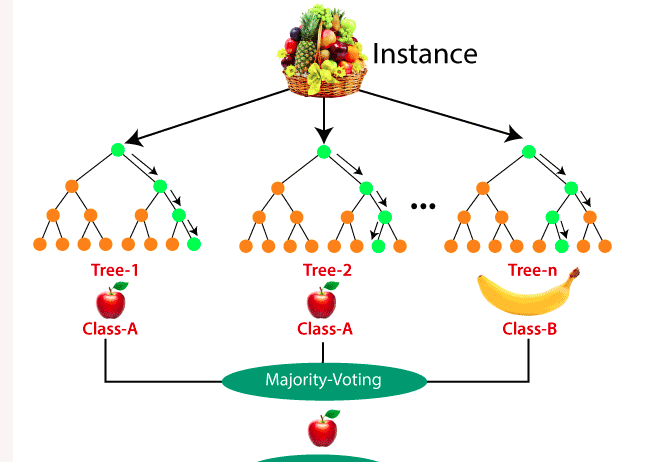
\includegraphics[width=14cm]{images/foret.png}
      \caption{Forêt aléatoire.\label{fig:foretaleatoire}}
    \end{center}
  \end{figure}


   \subsubsection{Echantillonage aléatoire des données d'entrainement}

    Lors de la phase d'entrainement, chaque arbre d'une forêt aléatoire apprend
    à partir d'un échantillon aléatoire de données. Les échantillons sont tirés 
    avec remplacement, connu sous le nom de \og bootstrapping \fg, ce qui 
    signifie que certains échantillons seront utilisés plusieurs fois dans un 
    seul arbre.

    Les prédictions sont faites en faisant la moyenne des prédictions de chaque
    arbre de décision. Cette procédure est connue sous le nom de \textit{bagging}
    abbréviation de \textit{bootstrap aggregating}

   \subsubsection{Fractionnement des noeuds}

    Le deuxième concept principal de la forêt aléatoire est que seulement un
    sous-ensemble de toutes les caractéristiques est pris en compte pour 
    diviser chaque noeud d'un arbre de décision. Cette valeur est 
    habituellement la raçine carré du nombre de caractéristiques pour une
    classification. Ainsi si nous avons 25 caractéristiques seulement 5
    seront pris aléatoirment pour diviser le noeud.

  \subsection{Les hyperparamètres dans les forêts aléatoires}

  Les hyperparamètres de la forêt aléatoires sont utilisés pour augmenter le
  pouvoir prédictif du modèle, soit pour rendre le modèle plus rapide.

  \subsubsection{Augmenter le pouvoir prédictif du modèle}

  Plusieurs hyperparamètres permettent d'augmenter le pouvoir de prédiction du
  modèle;
  \begin{description}
    \item[n\_estimators: ]Il s'agit du nombres d'arbres que l'algorithme
      construit avant de prendre le vote maximum ou la moyenne des prédictions.
      En général, un nombre d'arbres élevé augmente la performance et rend les
      prédictions plus stables mais ralentit également le calcul.
    \item[max\_features: ]Il s'agit du nombre maximum de caractéristiques qu'une
      forêt aléatoire considère pour diviser un noeud.
    \item[min\_sample\_leaf: ] Il s'agit du nombre minimum de feuilles nécessaires
      pour diviser un noeud interne.
  \end{description}

  \subsubsection{Augmenter la vitesse d'exécution du modèle}

  Les hyperparamètres permettant d'accélérer le modèle sont les suivants:
  \begin{description}
    \item[n\_jobs: ] Il indique au moteur le nombre de processeurs qu'il est autorisé
      à utiliser. Une valeur de $-1$ signifie qu'il n'y a aucune limite sur le
      nombre.
    \item[random\_state: ] Il rend la sortie du modèle reproductible. Le modèle
      produira toujours les mêmes résultats si on lui donne les mêmes
      hyperparamètres et les mêmes données d'entrainement.
    \item[oob\_score: ] Il s'agit d'une méthode de validation croisée des forêts
      aléatoires. Dans cette échantillonage, environ un tiers des données n'est
      pas utilisé pour entrainer le modèle mais plutôt pour évaluer ses
      performances sans aucune charge de calcul supplémentaire.
  \end{description}


\subsection{Les avantages et les inconvénients du modèle des forêts aléatoire}

\subsubsection{Avantages}
\begin{itemize}
  \item Les forêts aléatoires permettent de surmonter le problème de
    sur-ajustement en faisant la moyenne ou en combinant les résultats de
    diffrents arbres de décisions.
  \item Les forêts aléatoires fonctionnent mieux sur un large éventail de
    données qu'un seul arbre de décision.
  \item Les forêts aléatoires présentent moins de variance qu'un arbre de
    décision unique
  \item Les forêts aléatoires possèdent une très grande précision.
  \item Les algorithmes de forêt aléatoire maintiennent une bonne prédiction
    même si certaines informations sont absentes.
\end{itemize}

\subsubsection{Inconvénients}
\begin{itemize}
  \item La complexité est le principal inconvénient des algorithmes de Random
    Forest.
  \item La construction de forêts aléatoires est beaucoup plus
    difficile et longue que celle des arbres de décision.
  \item Il faut davantage de ressources de calcul pour mettre en oeuvre
    un algorithme de forêt aléatoire.
  \item Il est moins intuitif dans le cas où nous disposons d'une grande
    collection d'arbres de décision.
  \item Le processus de prédiction utilisant les forêts aléatoires est très long
    par rapport aux autres algorithmes.
\end{itemize}



